% \documentclass[conference]{IEEEtran}
\documentclass[journal]{IEEEtran}

\usepackage{xspace}
\usepackage{comment}
\usepackage{float}
\usepackage{graphicx}
\usepackage{multirow}


\begin{document}
%%%%%%%%% 
\markboth{COMP/ELEC 529 - Computer Network Protocols and Systems,
Project Proposal, Spring 2014}{right head} 
%Title
\title{Decentralizing the Internet}
\author{Adriana Flores, Clayton Shepard, Ellis Giles, Haihua Shen, Yanda Lu \\
Rice University
}
\maketitle
% \newcommand{\sys}{X\xspace}

%\today \\
\begin{abstract}
We propose to build and investigate a novel decentralized internet architecture in which servers are replaced with point to point communication for personal communication and services. %whenever possible.
Previously, servers have been a necessary part of the Internet to act as intermediaries between people who didn't have pervasive connectivity.
With the wide-spread adoption of smart-phones and wireless data, this antiquated paradigm is becoming less and less necessary, since there is no technological reason that devices can't connect directly to one another.
Indeed, there are many potential advantages to decentralizing the Internet, including security, privacy, resilience, cost, and power.
However, this novel decentralized architecture also presents many challenges, such as redundancy, uptime, and failover.
In this course project we will build a first generation decentralized Internet framework and address some of these challenges, as well as explore the unique opportunities, presented by this architecture.
\end{abstract}

\section{Introduction}
\label{Introduction}
In the early days of the Internet it was incredibly rare for normal users to have persistent, always-on connections.  
This limitation was addressed by servers, computers that were always on and always connected to the Internet, which served as an intermediary for communication between users.  
This server-client paradigm shaped the architecture of the Internet, and still dominates web communication today. 

However, with the penetration of always-on broadband and data-enabled cell-phones, coupled with the emergence of IPv6, which includes mobile IP, there is no longer a technological limitation which requires servers.  
The computers in our pockets have over a 99\% uptime and connectivity~\cite{rahmati2007context}!  
Indeed, centralized servers have many drawbacks, ranging from privacy, security, and fault-tolerance, to even energy-efficiency and control over data. 
An example centralized system is shown in Figure~\ref{Fig.Centalize}.
By decentralizing the Internet we could make it much robust to failure, much more secure; furthermore we could do away with many energy-hungry server-farms, and reclaim control of personal data. 
An example decentralized system is shown in Figure~\ref{Fig.Decentalize}.

While the idea of using our phones as personal servers is rather straightforward, it still raises many technical barriers.  
How do we ensure reachability?  
What happens if the cell-phone loses connectivity?  
What if it is lost/broken/stolen?  We need to find novel methods to ensure redundancy for both uptime and data.  
To address these issues we propose building a small cluster consisting of your personal devices (home computer, laptop, even router) possibly combined with friends’ and family devices to guarantee reliability and connectivity.

In light of this, we propose to build a first generation decentralized architecture which supports typical personal communication and applications including:
\begin{itemize}
  \item Email
  \item Web Pages
  \item Social Networking
  \item Chat
	%\item Voice Calls (VoIP)
\end{itemize}

\begin{figure}[h]
	\begin{center}
	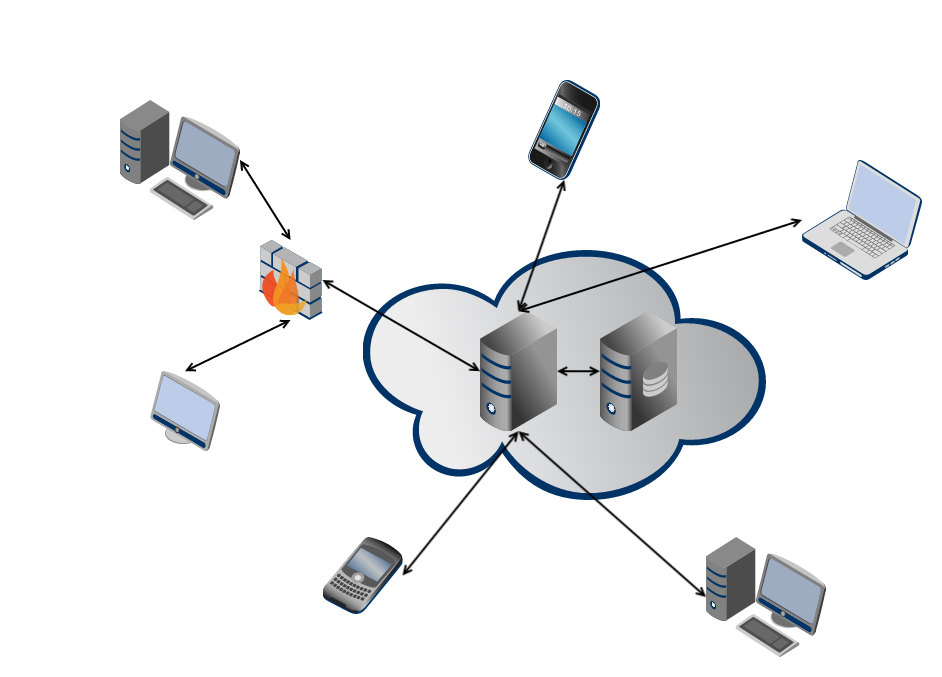
\includegraphics[width=2in]{centralized.png}
	\caption{ Centralized internet architecture.}
	\label{Fig.Centalize}
	\end{center}
\end{figure}
\begin{figure}[h]
	\begin{center}
	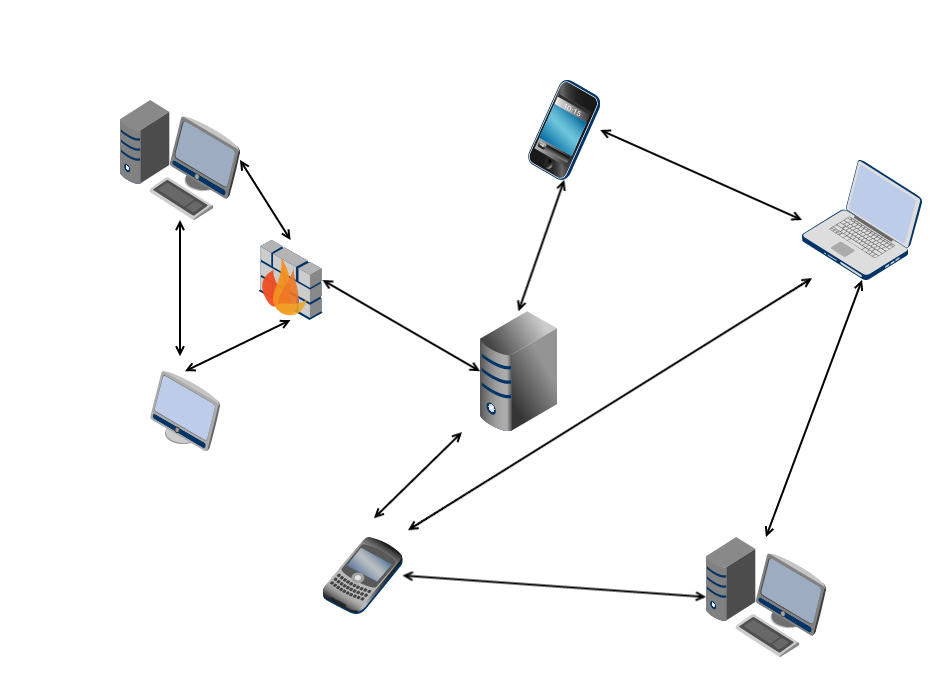
\includegraphics[width=2in]{decentralized.png}
	\caption{Decentralized internet architecture.}
	\label{Fig.Decentalize}
	\end{center}
\end{figure}

\section{Related Work}
\label{Related Work}

\subsection{Decentralized Internet}
%Haihua
%I haven't used Latex before and I don't have it installed right now. Would someone please help me translate the following paragraph into Latex syntax? Thanks! -Haihua
Decentralized Internet is a hot topic for network researchers. From the application perspective, centralization and decentralization each has advantages and disadvantages ~\cite{schuff2001}. 
Some of the more recent works have been done to provide alternative decentralized solutions for online social networks. 
For example, ~\cite{persona} proposed a decentralized version of Facebook to enhance privacy, and ~\cite{xu2010} suggested a P2P version of Twitter to improve scalability and reliability. 
In January 2014, a new project called Bitcloud was launched by the Bitcoin developers, seeking the possibility to decentralize the current Internet in order to improve privacy, security, and solve other current problem (like censorship) in today's centralized network.
Our goal is to investigate the possibility to use our phone as decentralized storage to support applications in a decentralized network. 
To achieve our goal, we would need to look into a variety of issues, such as the trustworthiness of storage, the reliability of communication, and the ability to recover from single-device failures.

\subsection{Data Replication}
%Ellis
Data replication and consistency are important aspects of any system where the availability and reliability of systems services are important.
Additional concerns such as scalability, performance, and fault tolerance play a role in deciding the best methods for data replication.
Data may be replicated at either file or data block levels, each presenting a unique set of challenges.
Considerations such as the network partition size, update frequency, replication granularity, number of users, security, reliability, and mobility all affect choices on the data replication policy.

Data replication in distributed systems, such as a Peer-To-Peer systems, where nodes are unreliable, additional considerations for the dynamic nature of nodes and data replication must be considered \cite{DRP}. 
Plover \cite{PLF} is a low-overhead file replication scheme for P2P networks that makes copies of files among physically close nodes based on capacities.
Decentralized P2P file sharing programs such as Limewire, Bittorrent, Kazaa, etc. replicate file data on end nodes, which may become corrupt or suffer from loss of availability.

Replica files are copies of a master file in a file replication system.
Files are replicated along data paths to reduce hot spots and improve efficiency.  A file replication algorithm that achieves high query efficiency at a low query cost for decentralized file sharing systems has been developed \cite{EAD}.
Demand based file replication and consistency by means of a group of File Replication Servers (FRS) \cite{DBF} has been explored which push data to other FRS when a requesting node requests a file.
PAST \cite{PAST} and CFS \cite{CFS}, a wide-area Cooperative File System, replicate files on nodes close to the owner of the file.  While PAST stores whole files, CFS replicates data at the block level to distribute the load and storage space among servers in the network.
CFS also uses Chord \cite{chord}, a scalable P2P lookup protocol for Internet Applications, to maintain routing tables used to find blocks.

Web applications often benefit from data replication of application data by low latency access and reduced network traffic.
Edge service delivery of content such as Content Delivery Networks (CDNs) like Akami typically cache static pages at end nodes and deliver them to customers from physically closer nodes, reducing overall latency.
GlobeDB \cite{GDB} automatically replicates Web application data.  It does not replicate web pages, but rather the underlying data in the web application database allowing for a Web application to be rendered at end nodes.
Distributed object caches such as MTCache, DBCache, and Memcached, are key-value stores that can also store the results of database queries as the value of the query key and allow for data replication for Web applications.
 

\subsection{Connectivity}~\label{sec:relconn}
%Clay
A key requirement for this architecture to be possible is pervasive connectivity and \emph{reachability}.
It is not enough for the device to have internet connectivity, but it must also be reachable from the internet.
This is a key challenge for our project, since almost all cell phone providers and WiFi access points hide their clients behind network address translation (NAT) and or a firewall which blocks reachability from the internet.
A lot of work has already been done on ensuring reachability, with the key technologies being IPv6, which includes Mobile IP, ~\cite{deering1998internet} as well as the Unmanaged Internet Architecture (UIA) project~\cite{ford2008uia, ford2006persistent}.

One of the primary motivations for using NAT is the scarcity of IPv4 addresses, as it allows multiple devices to connect to the internet through one public IP address.
IPv6 solves this limitation, as it has $7.9 \times 10^{28}$ times as many addresses as IPv4.
Additionally it includes Mobile IP, which allows devices to be located and contacted by their "`home address"' regardless of where the are on the internet.

Another very relevant project is Unmanaged Internet Architecture (UIA), as it seemingly solves the connectivity and reachability issue even in the current state of the internet, however it requires some assistance from devices with public IPs to enable NAT traversal.
Additionally it provides other very relevant services such as security, group management, overlay routing, and personal naming.

In short, while connectivity is an important part of our project, it seems that it is largely a solved problem, and thus will not be our focus.
While it is unlikely cellular provides will enable public reachability to cell phones, this is due to business and security reasons rather than a technological limitation.
% Note: I just came across Bitcloud [3], which deserves to be mentioned here as
% well.  I haven’t had a chance to look at it closely; while it looks to have
% similarities, it seems its goals and implementation are quite a bit different
% than what I’m proposing.


\subsection{Security}
%Adriana
A key concern when decentralizing the Internet is the storage and distribution of data among peers and friends. 
Trusting other devices with our personal data causes uncertainty, specially regarding integrity and privacy of the data. 
There exist vast previous work in data security, however we would to focus in secured distributed systems and data storage.
In distributed systems, there is no central system to protect, thus all nodes must collaborate to ensure security \cite{sit2002security}. 
A common approach of these systems is the peer-to-peer distributed hash lookup systems \cite{ratnasamy2001scalable, rowstron2001pastry, stoica2001chord}, in which lookups for keys are performed by series of nodes and forwarded to the node ultimately responsible for the key \cite{sit2002security}. 
Overall, approaches to ensure confidentiality, integrity and availability (CIA) must have capabilities of encryption, stringent access controls to data, backup and safe storage of data \cite{kaufman2009data}.

\subsection{Peer-Peer}
%Yanda
A common method to activate peer-peer communication, is the utilization of hashmaps. 
In our project peer to peer communication is based on a secure cluster which includes our trusted devices, thus a hashmap only includes the reachable and trustful devices. 
Existing hashmaps implementation works as follows.
Every time the device detects a new reachable device, it will put this divide into its own hashmap. 
And every time a device receives a message, it will look up the destination in its hashmap, if the destination is not found, it will make a connection with the destination. 
If it cannot, it will flood the message until get a signal of success. 
If it cannot receive a success signal for a period of time, maybe be 5 milliseconds, it will send the signal to the central server.
In contrast to this approach, our system will not depend in a central server.
There exist a plethora of current P2P frameworks such as Chord, Pastry, PAST, Tapestry, and Viceroy ~\cite{LUAsurvey}.
% 
% In our project, the devices cannot only have the ability to access to the Internet but also can access to other devices. 
% This technology refers to Peer-to-Peer, or P2P, but is not restricted solely to P2P. Because our project is based on a secure cluster which includes our trusted devices, we need to figure out some mechanics to implement the secure P2P.
% After reading some papers, we can put a hashmap on each device. The hashmap includes the reachable and trustful devices. 
% Every time the device detects a new reachable device, it will put this divide into its own hashmap, otherwise it will do nothing ~\cite{LUAsurvey}. 
% And every time a device receives a message, it will look up the destination in its hashmap. If it can find the destination, it will make a connection with the destination. If it cannot, it will flood the message until get a signal of success. If it cannot receive a success signal for a period of time, maybe be 5 milliseconds, it will send the signal to the central server.
% There exsit a plethora of current P2P frameworks such as Chord, Pastry, PAST, Tapestry, and Viceroy ~\cite{LUAsurvey}.
%In conclusion, we need to implement a secure peer to peer. It is not a difficult thing based on current technology, but we really need to do some things to completely implement it. 
\section{Methodology}
\label{Methodology}
The realization of our architecture can be divided in to two distinct stages: First we will leverage existing technologies to establish the framework for our system, in particular connectivity, reachability, and basic services.  
Second, we will build new technologies and applications to provide the key functionality of our decentralized system.

\subsection{Framework}
% Our framework can be divided in to two stages.  
% The first stage leverages existing "`off-the-shelf"' technologies to provide the foundation of our architecture.
% The second stage involves developing new technologies and applications to provide the key functionality of our decentralized system.
% 
%\subsubsection{Foundation of Exisiting Technologies}
The first step in realizing our architecture is establishing connectivity and reachability to our devices.
As discussed in Section~\ref{sec:relconn}, existing work has already addressed, and largely solved, this issue, thus it will not be our focus.
Unfortunately these methods have not been widely deployed, are blocked, or have only been tested in lab settings.
%While there are existing technologies which address this issue, as discussed in Section~\ref{sec:relconn}, these methods have not been widely deployed, are blocked, or have only been tested in lab settings.
%Since this is not our area of focus, we 
To bypass this challenge, we intend to use a VPN server, such as OpenVPN~\cite{feilner2006openvpn}, running on an RECG lab server to allocate static public IPs to our devices.
We hope that this will enable our devices to be publicly accessible, as well as provide a reliable way for them to communicate with each other.
However, if this approach fails, we may have to fall back to other methods such as UIA~\cite{ford2008uia,ford2006persistent}, or limit the scope of our experiments.

The next component in our architecture is device naming and management.
Conventional DNS provides human friendly names as well as domain management, and, in more advanced systems can also provide load-balancing and failover.
In our architecture we will additionally use it help specify our personal "`mini-clusters"' and failover order.
For example, each group member will have their own sub-domain, then further sub-domains will be used to manage that users' devices and cluster.  Figure ~\ref{Fig.Venn} is an example of a possible namespace.
More specifically we intend to use a name such as "`phone.adriana.recg.rice.edu"' or "`laptop.adriana.recg.rice.edu"' to point to Adriana's phone and laptop respectively, then perhaps "`failover1.adriana.recg.rice.edu"' up to "`failoverN.adriana.rice.edu"' to specify the N failover devices in Adriana's cluster.
Similar naming would be used for each persons' cluster.
Notably these names would only be used internally, and would not be seen by the users.
While DNS is a centralized service, thus breaking our decentralized mantra, we use it out of convenience and time considerations; other decentralized naming systems could also be used similarly, such as the one proposed in UIA.

\begin{figure}[h]
	\begin{center}
	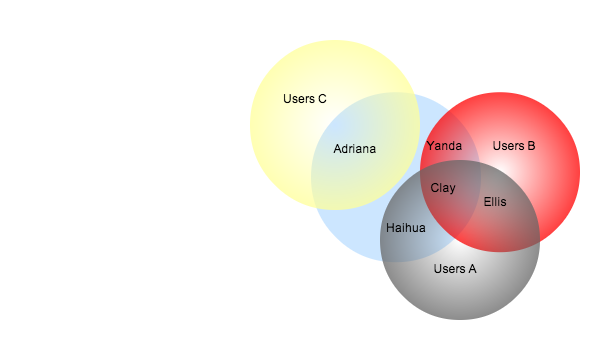
\includegraphics[width=2.5in]{venn.png}
	\caption{Example Namespace.}
	\label{Fig.Venn}
	\end{center}
\end{figure}

The final "`off-the-shelf"' component of our framework is open-source server software, such as postfix, sendmail, apache, etc., which will provide the basis of our communication services.
Combined with the reachability and naming described above, this provides a complete framework for our decentralized framework, which should provide full communication and service, which are even backwards compatible with the existing email and web services.
However, this framework lacks two key features: redundancy and failover.
Additionally, this framework provides some unique opportunities for optimization, which we elaborate on below.
\begin{comment}

%note from Clay:  This is good, but it's probably getting a bit too detailed, especially since a lot of it we either won't be using, or is fairly standard.  Our VPN should take care of all of this since it will assign public static IPs, though DyDNS and UIA may be good to mention as fallbacks.
%Yeah, it's more background stuff.

%The Internet Domain Name Systems (DNS) provides a method for addressing computers based on host or computer names that resolve to specific IP addresses. 
%DNS also allows for directory like services such as Alias or Canonical Names, and services such as Mail Exchange records.   
%Additionally, multiple IP addresses might be configured to correspond to a single host name entry, which helps provide for fault tolerance and load balancing.
%Though the Time-To-Live, or TTL, of a record can be set to zero, numeric IP address changes for a specific DNS record must be updated manually.
%Dynamic Host Configuration Protocol (DHCP) allows for hosts to obtain dynamic IP addresses when they are connected to the network, but this can lead to problems with DNS entries as an IP address might change.
%Dynamic DNS, however, provides a means for automatically updating the DNS record of a host when the host’s IP address changes.
%This is accomplished by using a small piece of software on the host computer that periodically notifies a DNS server of the host’s IP address.
%Such Dynamic DNS providers include DNS Dynamic, Change IP, No-IP, Dyn-DNS, and Zone Edit.
%In UIA, the requestor leases a name entry from a responder for a certain period of time.
%The responder can then notify the requestor when the underlying IP address changes.
%Additionally, the devices in UIA operate in an overlay routing protocol so that changes in IP addresses or Network Address Translation can be resolved into location independent connectivity \cite{ford2008uia,ford2006persistent}.
%Virtual Private Network connections allow a computer to utilize a network as if it were connected directly to the network, even when it is on another network.
%A VPN can provide local IP addresses to the network as well as access to local services.
%Mobile IP is an open standard that can give a mobile device the appearance of having a static IP address even when the device changes to a new network and gets a new physical IP address.  It works by devices having a Home Agent that forwards information to the mobile device through a Foreign Agent when the mobile device is not on the home network.

 DNS
 VPN
 Public IP
 Open source
 
 1 Server with public IPs
 
 2 installing server email...
 
 3. setup DNS 
 
The first stage of this project would be to install (or perhaps port)
open-source server software, e.g. Apache, Jetty, postfix, sendmail, etc., to a
phone.  The next stage would be to ensure reachability from the Internet.  Some
work has already been done here, such as UIA [2]; however, since IPv6 and
MobileIP already address this issue,

it may be best to focus on other challenges
which are more novel.  In the meantime we could use a custom APN (which Rice may
already have), or VPN, to assign a public IP to the phones.  The final research
stage of the project could take one of many directions including ensuring data
redundancy, uptime measurements, distributing loads, power consumption,
encryption, etc.  Perhaps, since this is a networking course, the focus should
be on how to maintain seamless connectivity on node failure in such a system
(beyond simple DNS failover).
\end{comment}
%
%
\subsection{Performance Metrics and Analysis}
Once we have built our decentralized architecture, it is critical to analyze its performance.
We will analyze:
\begin{itemize}
 \item Uptime, Reachability, and Failover
 \item Failure Resistance and Recovery
 \item Load balancing and power efficiency
\end{itemize}

\subsection{Key Issues}
Even when building a decentralized architecture, we are still required to provide reliability by having 100\% availability of the data and fast accessibility. 
In order to achieve the goals of reliability, 100\% availability and fast accessibility, our system must overcome the following.

\textbf{Failover.}  %note from Clay:  actually it is quite the opposite -- there is no signle point of failure in a decentralized system... that is one of the main advantages we are arguing for.
%the issue is just detecting the failure and moving on to the next device in line to accept the request.
% Yes that is the point I was trying to make, let me reword.
In a decentralized architecture, the number of point of failures are increased. 
In a centralized architecture, if a central server fails, it is easily trackable and detectable.
However, in the case of a distributed architecture, the points of failure are multiplied. 
Even though, multiple point of failures is helpful in security purposes, it makes the system more prone to errors because detecting the failure is harder to then activate failover mechanism.
In order to address this issue, our system relies on data replication or redundancy. 
Data will be distributed across multiple nodes, where we will provide a redundancy level that is proportional to the size of the network and load.

Furthermore, we identify there exist varying requirements in failover strategies for different applications. 
In the case of real-time applications, such as chat or VoIP, if the user is unavailable or offline, there is no necessity in activating failover to other people's devices. 
Instead, failover for real-time applications should occur between the devices of the same owner. 
For example, if my phone is unavialble, my calls can failover to any other of my active devices.

In general, by storying multiple copies of the data our system will combat failovers. 
Moreover, our system will consider application base failover possibilities. 
Furthermore, as explained bellow, our system will take into consideration device capabilities for data distribution, thus reducing the possibility of failovers from power outage or other device dependent issues.

\textbf{Diversity in Device Capability.}
Since, data will be store in various types of devices, our system is required to be robust to the different device capabilities. 
A key example of diverse capability is power or battery life. Some devices might be able to have longer up-time than others, thus our system is required to adapt to such differences. 
A possible approach is power adaptation, by analyzing remaining battery life of a device, to then perform decisions of reducing transmission power or even remove such device from the cluster. 
Another example of diverse capability is the storage capability of a device. Some devices might be capable of storing larger amounts of data than others. 
Overall, our system will approach different device capabilities by analyzing each device, building a feedback infrastructure and performing decisions based on each device capability. Through this we ensure data distribution is performed properly in order to achieve our goals.
% 
%Clay: an interesting thing to note here may be the privacy issue.  While the decentralized architecture is more private from a "`big brother"' aspect, it seems that in many other cases it may be a huge problem, as many of the things we want kept private are from our friends/family (whereas we don't necessarily care if google knows).  
% For example, say I have a doctors appointment that I don't want my friends to know about, but my device goes offline, and the email gets sent to their device.  
% Obviously the system doesn't intentionally tell the friend I just received an email from my doctor, but it would be trivial for them to figure it out...  (even if it were encrypted using something like pgp, it wouldn't hide the sender's IP...)  Maybe we can find a way around this?
% 

\textbf{Mode of Connectivity.}
Different modes of connectivity will be supported and tested for different devices.
For instance, a mobile phone could connect to the framework using a Wi-Fi connection direct to local network services.
Alternatively, it could connect using a VPN through a cellular telephone network.
Ideally, the device should make a connection that supports the best overall user experience for the device user as well as the users consuming services provided by the mobile device.  Bluetooth would be another possible connection mode, but is probably beyond the scope of this project.   Laptop devices could connect in a wired or wireless fashion to the framework. Each connectivity method would consume a different set of resources and provide a different level of service.  In our project we would like to not only make the method of connectivity as easy as possible for the end user, but will also measure the performance tradeoffs of connectivity modes.
\begin{comment}
For our project, the mode of connectivity should be wireless combining with wire. 
The desktop computers use wire connecting with the AMAZON EC3, but the rest parts use wireless connecting with each other. 
Bluetooth is an alternative connectivity, but we think it cannot be used very commonly. Not each device will turn on the bluetooth because of the easily consumption of battery. 
In conclusioin, the mode of connectivity based on wireless between different operating system, like mobile system for Andriod and iOS and desktop system for Windows and MAC OS X.
\end{comment}
\section{Expected Outcomes and Schedule}

\subsection{Expected Outcomes}
% In our project we plan on
% 
% we plan on developing an app that will address or automate tough problems in decentralizing the internet....  
% Framework, we plan on developing a framework to address the problems with changing ip addresses.....
The expected outcomes of our project can be divided into four stages. In stage 1, we plan to identify, install and deploy our framework with off-the-shelf technology (VPN server with public IPs and DNS) to meet our basic needs. 
Next, in stage two we plan to extend our framework beyond off-the-shelf technologies in order to ensure the framework is capable of executing all our needs in terms of analysis and system features.
Third, we will integrate use cases to our framework, meaning we will deploy applications that will allow us to test our system. Example applications we consider in deploying are wordpress or open source source social media.
In the last stage, we plan to test and analyze performance of the system in terms of failover, power and other device capability dependent issues. 

\subsection{Schedule}
\begin{itemize}
 \item Beginning March - Framework Setup: Get connectivity and reachability on phones (VPN server with public IPs and DNS)
 \item Early March - Framework Setup: Servers installation (Web and Email)
 \item Mid March - Midterm Presentation: We will have basic experimental framework installed so we can start working on novel issues (replication, failover, and power).
 \item Ending March - Data Replictaion: Basic replication scheme working
 \item Early April - Failover: Basic failover mechanism developed and implemented
 \item Mid April - Power: Experiment with performance and power
 \item April 22- Final Report: Integrate results into the final report
 \item April 22 - Final Presentation: Polish and integration into ``app`` 
\end{itemize}



%%%%%%%%%  References
\bibliographystyle{IEEEtran} %S sort alfab.
% \bibliography{IEEEabrv}
\bibliography{References}

\end{document}
